\section{Signing the JAR Files}

In order to run the Java RIA we had created, we had to export as a JAR and sign with out x509 certificate. Signing with our certificate essentially states that we verify using our certificate that the applet is trustworthy, a user can choose to accept our declaration by be importing the corresponding CA into the 'Signer CA' section of the Java Control panel. We were also required to sign the Bouncy castle Jars as well. Below is screen shots providing the steps that we went through.
\newpage
\noindent Exporting as a JAR

\begin{figure}[hbt!]
	\centering
      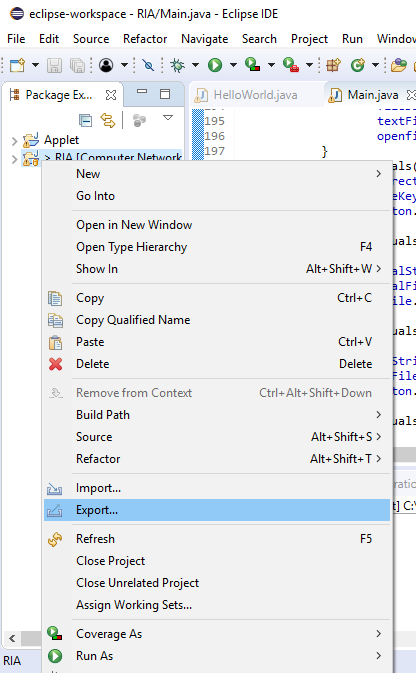
\includegraphics[width=0.4\textwidth]{imgs/jarsign/export} \\
	\caption{Exporting as JAR file}
	\label{fig:specifiyingkeysize}
    \noindent\makebox[\linewidth]{}
\end{figure}

\noindent Adding Manifest file

\begin{figure}[hbt!]
	\centering
      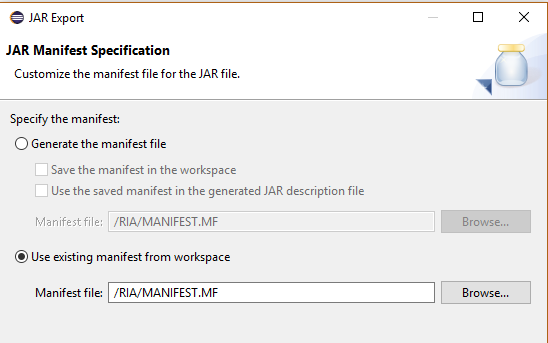
\includegraphics[width=0.4\textwidth]{imgs/jarsign/manifest_apply} \\
	\caption{Selecting manifest to add}
	\label{fig:specifiyingkeysize}
    \noindent\makebox[\linewidth]{}
\end{figure}

\noindent After exporting the JAR, we now signed it using jarsigner and our x509 certificate.

\newpage
\begin{figure}[hbt!]
	\centering
      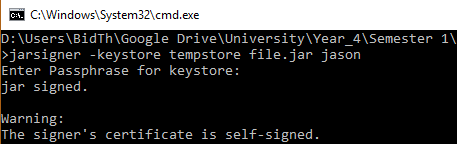
\includegraphics[width=0.4\textwidth]{imgs/jarsign/sign_applet_jar} \\
	\caption{Jarsigner}
	\label{fig:specifiyingkeysize}
    \noindent\makebox[\linewidth]{}
\end{figure}

